\documentclass[mathserif, 10pt, aspectratio=169]{beamer}
\usepackage[utf8]{inputenc}
\usepackage{amsmath, amsfonts}
\usepackage{appendixnumberbeamer}


\title{Light New Physics coupling to $\tau$}
\subtitle{{\bf JA}, G. Levati, P. Paradisi, S. Rigolin, N. Selimovic}
\author[Jorge Alda]{Jorge Alda \hspace{4em} \texttt{jorge.alda@pd.infn.it} \\
Università degli Studi di Padova \& CAPA}
\date[Saturnalia '23]{Saturnalia '23 \\ 21-12-2023}



\usetheme{Zaragoza}
\usecolortheme{Unipd}
\titlepagelogoA{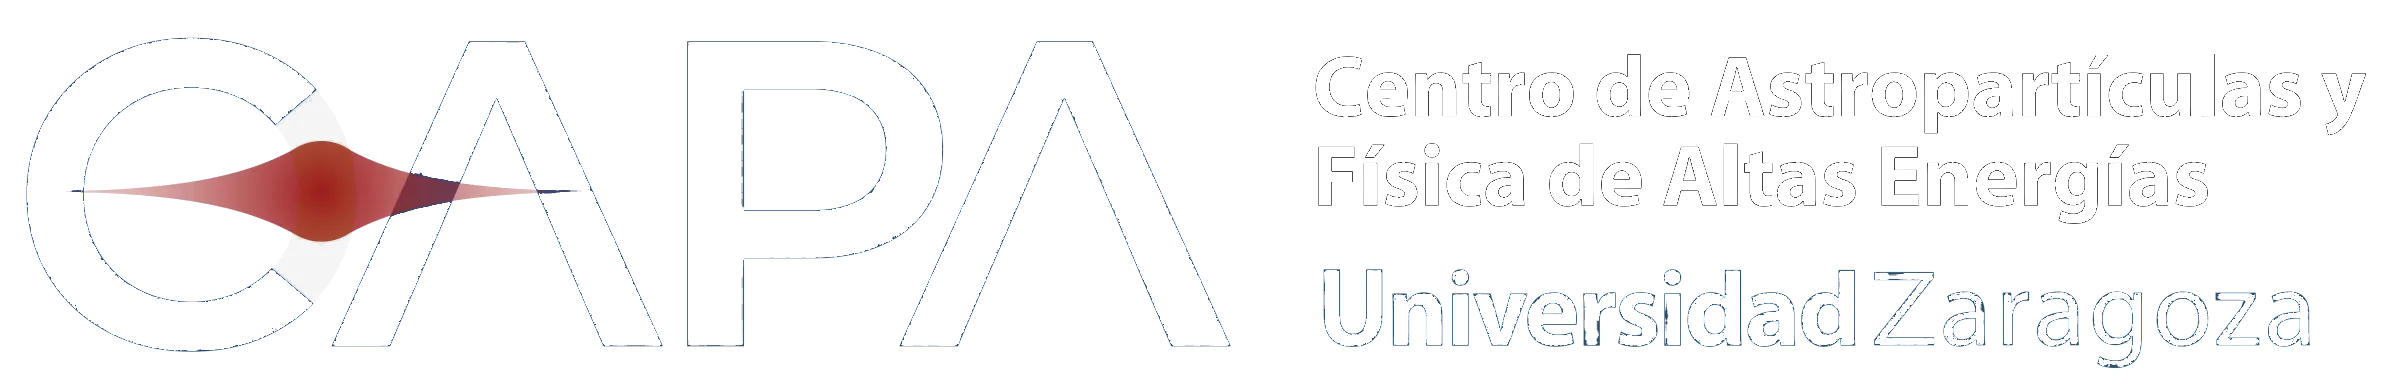
\includegraphics[width=4cm]{logos/CAPA.png}}
\titlepagelogoB{
\includegraphics[width=6cm]{logos/unipd.png}}




\begin{document}
\begin{frame}[noframenumbering,plain]

\titlepage

\end{frame}

\begin{frame}\frametitle{Why New Physics?}
    Our objective is to look for signs of New Physics, motivated by\vspace{20pt}
    \begin{itemize}\setlength{\itemsep}{10pt}
        \item Theoretical questions: Flavour puzzle, dark matter, dark energy, unification with gravity, hierarchy problem, etc.
        \item Experimental anomalies: $(g-2)_\mu$, $R_{D^{(*)}}$, Cabbibo anomaly, etc.
        \item Elaboration of hypotheses.
    \end{itemize}
\end{frame}

\begin{frame}\frametitle{Why Light New Physics?}
    \begin{itemize}\setlength{\itemsep}{10pt}
        \item We could see it in the current particle colliders in the form of resonances (``visible'' decays) or missing energy (``invisible'' decays).
        \item Also in other experiments: helioscopes, astronomical observations, etc.
        \item Can not be described as an Effective Field Theory.
        \item Theoretical motivation: Dark Matter candidates, Strong CP problem, axiverse.
    \end{itemize}
\end{frame}

\begin{frame}\frametitle{Strong CP problem}
    \begin{itemize}\setlength{\itemsep}{10pt}
        \item Three discrete transformations: Charge conjugation (C), Parity (P) and Time reversal (T).
        \item Experimentally, C, P and CP are not symmetries of the SM.
        \item Strong interactions preserve CP, although we could write a CP-violating term $\theta G\tilde{G}$.
        \item Very strong experimental bounds from electric dipole moment of the neutron.
        \item {\bf Peccei-Quinn mechanism:} A new pseudo-scalar field with anomalous couplings to gluons $a G\tilde{G}$ which develops a vev, dynamically erasing the CP violation. Its particle excitation is the axion.
        \item Characterized by energy scale $f_a$ and mass $m_a f_a \sim m_\pi f_\pi$.
        \item Shift symmetry $a \to a + \mathrm{constant}$.
    \end{itemize}
\end{frame}

\begin{frame}\frametitle{Axion-Like Particles}
    \begin{itemize}\setlength{\itemsep}{15pt}
        \item Many beyond-SM models propose a new global $U(1)$ symmetry, spontaneously broken at energies $f_a \gg v$. The Nambu-Goldstone boson (NGB) associated to this symmetry would be an Axion-like particle (ALP).
        \item If the symmetry is also explicitly broken, the ALP is a pseudo-NGB, and $m_a f_a \nsim m_\pi f_\pi$.
        \item As an example, string theory predicts the existence of many ALPs in a wide range of masses and energy scales as a result of the compactification of antisymmetric tensor fields.
    \end{itemize}
\end{frame}

\begin{frame}\frametitle{Why coupling to $\tau$?}
    \begin{columns}
        \begin{column}{0.6\textwidth}
            \begin{itemize}\setlength{\itemsep}{10pt}
                \item Many experimental constraints for couplings to photons and to quarks.
                \item The couplings to fermions are proportional to their mass, and $\tau$ is the heaviest lepton.
                \item New Physics in 3rd generation, consistent under RG flow.
                \item Improved experimental sensitivity to $\tau$ (e.g in Belle-II).
            \end{itemize}
        \end{column}
        \begin{column}{0.27\textwidth}
            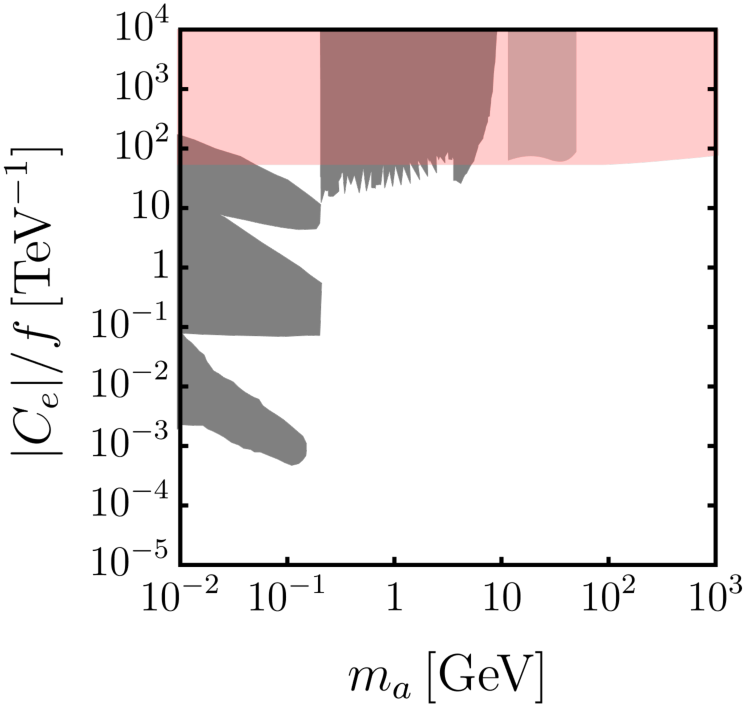
\includegraphics[width=\columnwidth]{figures/Neubert_Ce_Bounds.pdf}\\{\scriptsize A. Biekötter, J. Fuentes-Martín, A. M. Galda and M. Neubert, arXiv:2307.10372}
        \end{column}
    \end{columns}
\end{frame}

\begin{frame}\frametitle{Light New Physics}
    Axion-like Particle coupled to a Peccei-Quinn current of leptons

    $$\mathcal{L}_\mathrm{ALP} = \frac{1}{2}\partial_\mu a \partial^\mu a - \frac{1}{2} m_a^2 a^2 - \frac{1}{2 f_a}\partial_\mu a j^\mu_\mathrm{PQ}\,;$$

    $$j^\mu_\mathrm{PQ} = \sum_{i,j} \left( c_{\ell\ell}^{ij} \bar{\ell}_i\gamma^\mu \gamma_5 \ell_j + \bar{c}_{\ell\ell}^{ij} \bar{\ell}_i\gamma^\mu  \ell_j  + c_{\nu\nu}^{ij} \bar{\nu}_{\ell_i} \gamma^\mu P_L \nu_{\ell_j} \right)\,. $$

    $m_a \in [1\,\mathrm{MeV}, 10\,\mathrm{GeV}]$, $f_a \sim 1\,\mathrm{TeV}$, flavour-universal $c^{ij} = c \delta^{ij}$ or $\tau$-phillic $c^{ij} = c \delta^{i3}\delta^{j3}$.\\


    Electroweak-preserving case: $c_{\ell\ell} - \bar{c}_{\ell\ell} + c_{\nu\nu}=0$.
    \begin{center}
        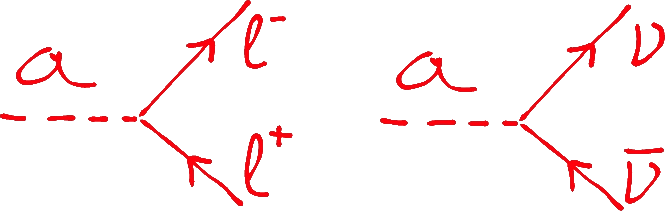
\includegraphics[width=0.45\textwidth]{figures/rules_derbasis.png}
    \end{center}
\end{frame}

\begin{frame}\frametitle{Light New Physics}
    After integration-by-parts and equations-of-motion
    $$\mathcal{L}_\mathrm{ALP, int} = \frac{a}{f_a}\sum_\ell \left(i c_{\ell\ell}m_\ell \bar{\ell}\gamma_5\ell  + \frac{ig}{2 \sqrt{2}} (c_{\ell\ell} - \bar{c}_{\ell\ell} + c_{\nu\nu}) (\bar{\ell}\gamma^\mu P_L \nu_\ell) W^-_\mu + \mathrm{h.c.} \right) + (V\tilde{V}a)\,.$$
    \vspace{10pt}
    \begin{center}
        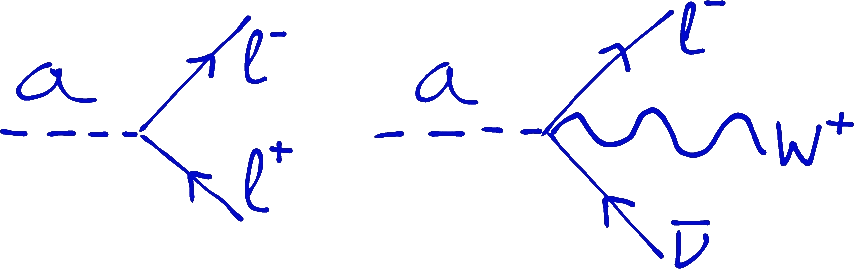
\includegraphics[width=0.45\textwidth]{figures/rules_Yukbasis.png}
    \end{center}
\end{frame}

\begin{frame}\frametitle{Particle decays}
    
    \begin{columns}

        \begin{column}{0.6\textwidth}
            The ALP particles can decay to a pair of leptons

            $$\Gamma(a \to \ell^+\ell^-) = \frac{m_a}{8\pi} |c_{\ell\ell}|^2\frac{m_\ell^2}{f_a^2} \left(1-\frac{4 m_\ell^2}{m_a^2}\right)^{1/2}\,,$$

            Also decays to $2\gamma$ through a lepton loop.

            ~

            ALPs with $m_a > 2 m_\mu$ will typically decay inside the detector.
        \end{column}
        \begin{column}{0.36\textwidth}
            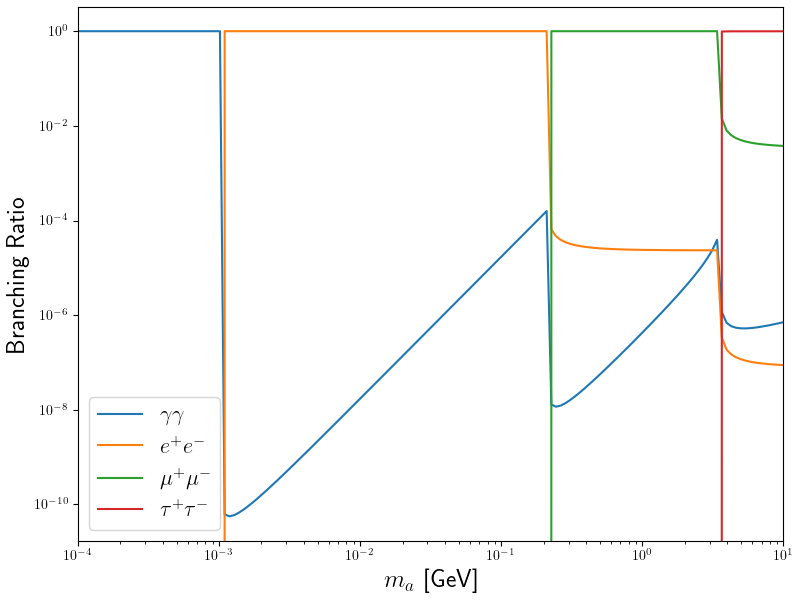
\includegraphics[width=\columnwidth]{figures/BR.png} \\
            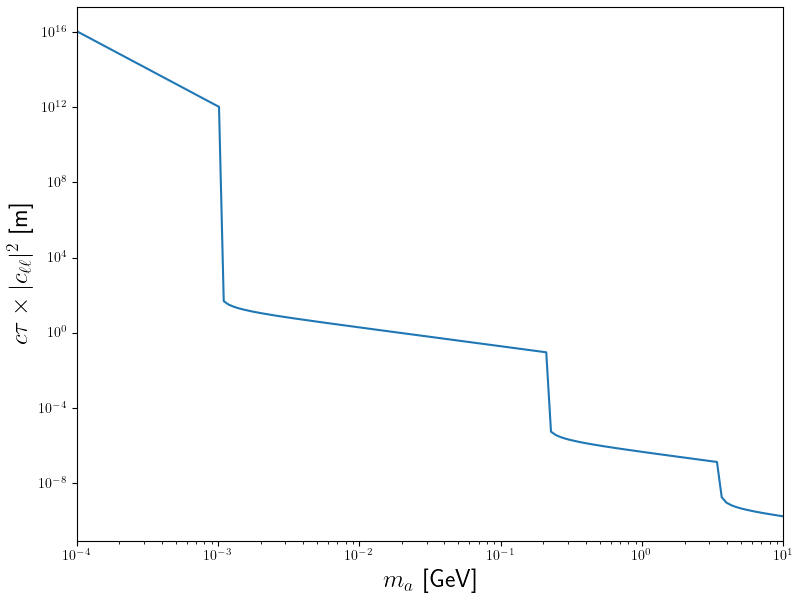
\includegraphics[width=\columnwidth]{figures/decaylength.png}
        \end{column}
    \end{columns}
\end{frame}

\begin{frame}\frametitle{Collider searches}
    Production of visible ALPs in Belle, Belle-II and FCC-ee: the ALP decays into a pair of lighter leptons inside the detector.
    \begin{center}
        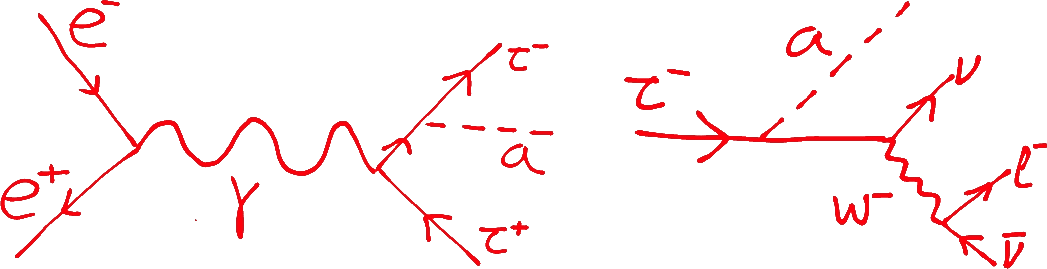
\includegraphics[width=0.65\textwidth]{figures/collider.png}
    \end{center}
    Bump searching at $m^2_{\ell\ell} = m_a^2$.
\end{frame}

\begin{frame}\frametitle{Leptonic $B$ decays}

    $B$-meson leptonically decaying into an invisible ALP.
    $$\frac{\mathrm{BR}(B^-\to \ell^- \bar{\nu}_\ell a)}{\mathrm{BR}(B^-\to \ell^- \bar{\nu}_\ell)} \approx \frac{1}{1536\pi^2}\frac{m_B^4}{m_\ell^2 f_a^2}\left[(c_{\ell\ell}-\bar{c}_{\ell\ell}+c_{\nu\nu})^2+\frac{16 m_\ell^2}{m_B^2} c_{\ell\ell}^2\right]$$

    \begin{columns}
        \begin{column}{0.55\textwidth}
            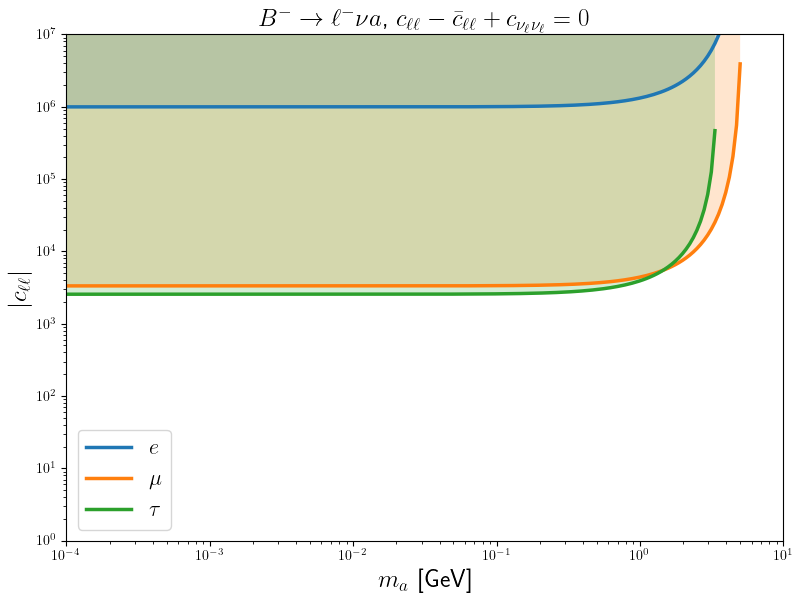
\includegraphics[width=\columnwidth]{figures/limcl.png}
        \end{column}
        \begin{column}{0.4\textwidth}
            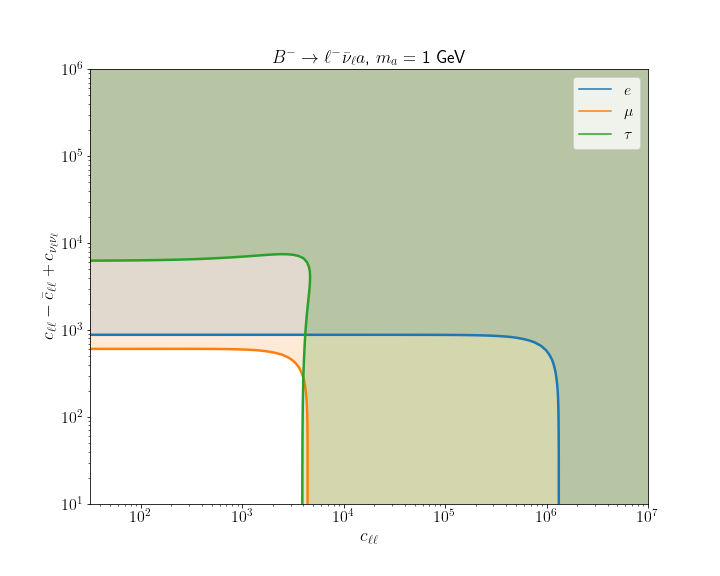
\includegraphics[width=\columnwidth]{figures/lim_c_1GeV.png}
        \end{column}
    \end{columns}
\end{frame}

\begin{frame}\frametitle{Gauge boson decays}
    \begin{columns}
        \begin{column}{0.5\textwidth}
            \begin{center}
                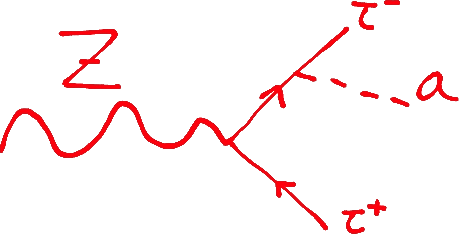
\includegraphics[width=0.4\columnwidth]{figures/diagZ.png}\hspace{5pt}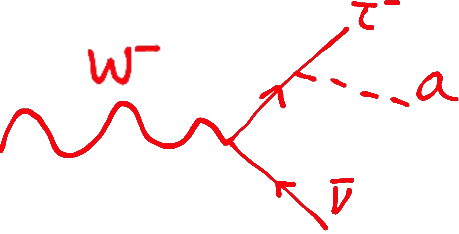
\includegraphics[width=0.4\columnwidth]{figures/diagW.png}
            \end{center}
            Production of invisible ALP in $Z\to \tau^+\tau^- a$ and $W^-\to \tau^- \bar{\nu}_\tau a$.

            For the $W$ decays there are additional terms in the case of EW-violating interactions.
        \end{column}
        \begin{column}{0.47\textwidth}
            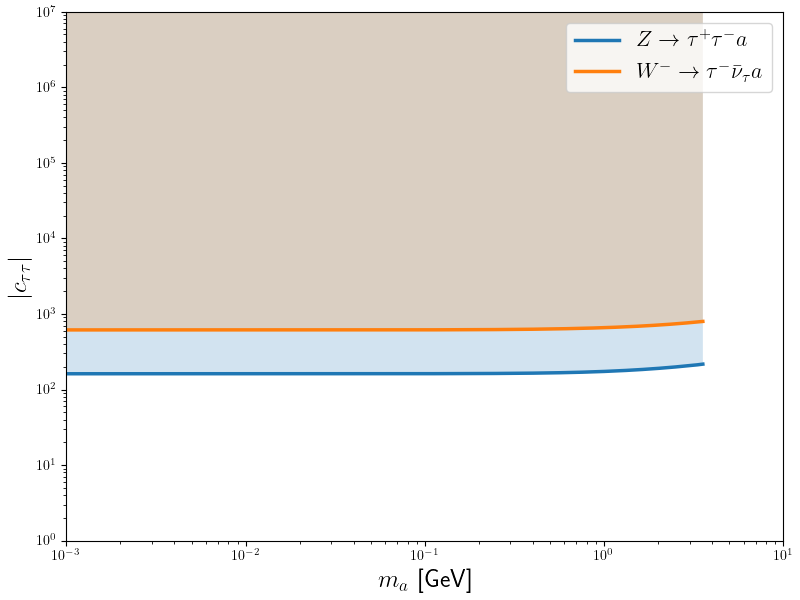
\includegraphics[width=\columnwidth]{figures/boson_decay.png}
        \end{column}
    \end{columns}
    
\end{frame}

\begin{frame}\frametitle{$(g-2)_\tau$}
    \begin{columns}
        \begin{column}{0.5\textwidth}
            \begin{center}
                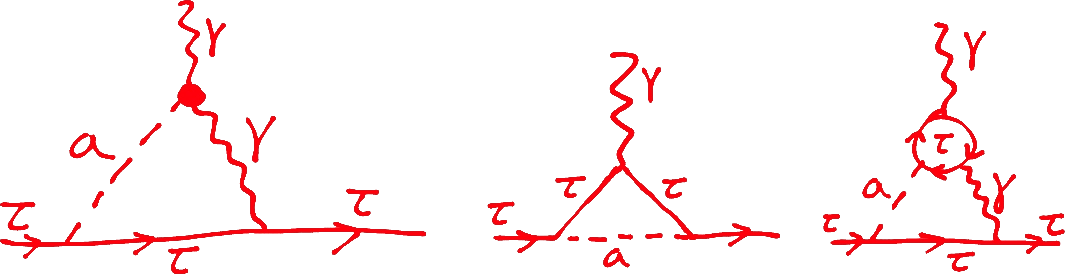
\includegraphics[width=\columnwidth]{figures/g2tau.png}
            \end{center}
            \begin{itemize}
                \item New (2022-23) measurements of $(g-2)_\tau$ at LHC
                \item Still not very precise ($|a_\tau|<1.8\times 10^{-3}$)
                \item  Belle-II is expected to achieve a precision of $\sim 10^{-6}$
            \end{itemize}
        \end{column}
        \begin{column}{0.47\textwidth}
            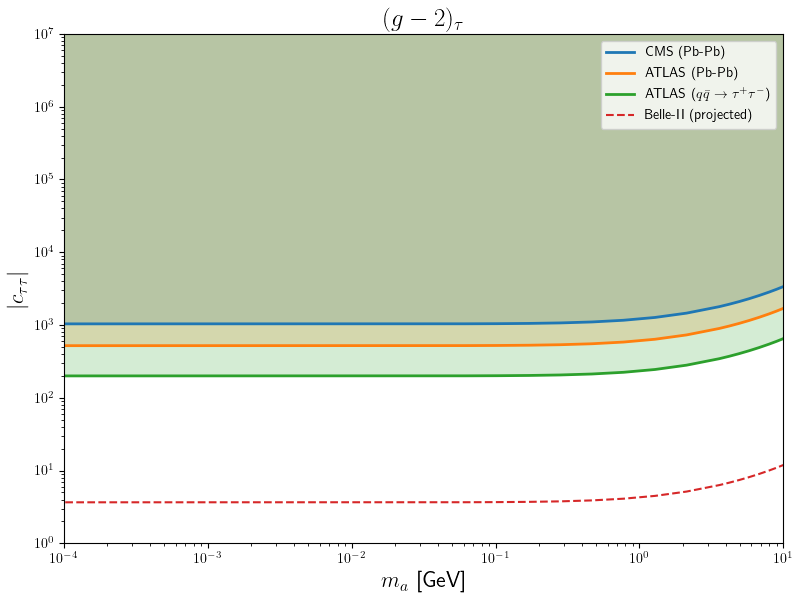
\includegraphics[width=\columnwidth]{figures/g2tau_lim.png}
        \end{column}
    \end{columns}
    
    
\end{frame}


\begin{frame}\frametitle{Bounds for couplings to $\tau$ leptons}
    \begin{center}
        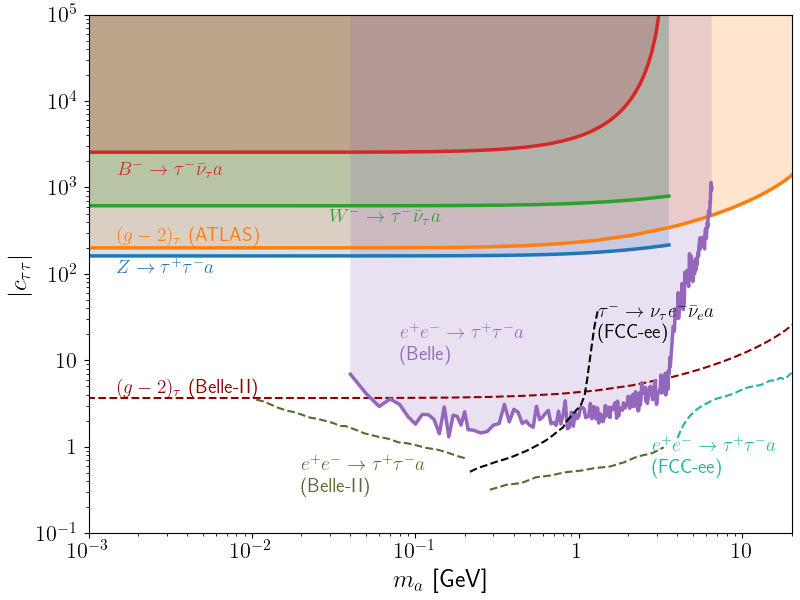
\includegraphics[width=0.75\textwidth]{figures/moneyplot.png}
    \end{center}
\end{frame}


\begin{frame}\frametitle{Conclusions}
    \begin{itemize}\setlength{\itemsep}{15pt}
        \item ALPs are a well-motivated extension of the SM with a new light pseudoscalar particle.
        \item We studied ALPs coupling to $\tau$, both in LFU and $\tau$-phillic scenarios.
        \item Production of ``visible'' ALPs in colliders:
        \begin{itemize}
            \item Dedicated search at Belle.
            \item Belle-II will improve the bounds, and FCC-ee will explore heavier ALP masses.
        \end{itemize}
        \item ``Invisible'' ALPs in $B^-\to \tau^-\bar{\nu}_\tau a$, $W^-\to \tau^-\bar{\nu}_\tau a$ and $Z \tau^-\tau^+ a$ complement direct searches for lighter ALPs.
        \item Loop effects in $(g-2)_\tau$, will drastically improve in Belle-II.
    \end{itemize}
\end{frame}

\begin{frame}\frametitle{Outlook}
    \begin{itemize}\setlength{\itemsep}{15pt}
        \item Still Work in Progress
        \item Invisible ALPs in $e^+e^-\to \tau^+\tau^- a$.
        \item $B\to D^{(*)}\tau^-\bar{\nu}_\tau a$ and $R_{D^{(*)}}$?
        \item Generalization to other light NP particles: scalars, dark photons, etc.
    \end{itemize}
\end{frame}

\begin{frame}\frametitle{Bibliography}
    \begin{itemize}\setlength{\itemsep}{7pt}
        \item JA, A. Guerrera, S. Peñaranda and S. Rigolin: ``Leptonic meson decays into invisible ALP''. Nucl.Phys.B 979 (2022) 115791, arXiv:    2111.02536 [hep-ph]
        \item W. Altmannshofer, J. A. Dror, and S. Gori, ``New Opportunities for Detecting Axion-Lepton Interactions'' Phys.
        Rev. Lett. 130 no. 24, (2023) 241801, arXiv:2209.00665 [hep-ph]
        \item D. Biswas et al. (Belle), ``Search for a dark leptophilic scalar produced in association with $\tau^+\tau^-$ pair
        in $e^+e^-$ annihilation at center-of-mass energies near 10.58 GeV'' arXiv:2207.07476 [hep-ex]
    \end{itemize}
\end{frame}

\end{document}